\documentclass[nochap]{apuntes}

%
\author{Guillermo Julián}
\date{C2 - 2011/2012}
\title{Cálculo II}
%

\begin{document}

\pagestyle{plain}
\maketitle
\newpage

\tableofcontents

\newpage

\section{Estructura de $\real^N$}

\subsection{Vectores}

Operaciones básicas: suma, producto por un número real.

\begin{defn}[Producto\IS escalar Euclídeo]
\[ \vx\cdot\vy=\pesc{x,\,y} = \sum_{i=1}^Nx_iy_i = \md{\vx}\md{\vy}\cos \alpha \]
\end{defn}

\begin{defn}[Norma\IS Euclídea]
\[ \md{x} = \sqrt{\vx\vx} \]
\end{defn}

La norma euclídea es mayor o igual que cero y cumple la desigualdad triangular.

\begin{defn}[Distancia\IS euclídea]
\[ D(\vx , \vy) = \abs{\vx - \vy} \]
\end{defn}

\begin{theorem}[Desigualdad\IS Cauchy-Schwarz]
\[\abs{\vx\vy}\leq\md{x}\md{y}\]
\end{theorem}

\begin{defn}[Ortogonalidad]
Dos vectores son ortogonales si el ángulo que forman es un ángulo recto:
\[ \vx\bot\vy \dimplies \cos \alpha = 0 \dimplies \vx\vy = 0\]
\end{defn}

\subsection{Sucesiones en $\real^N$}

Notación: $\{\vx_k\}_{k\in\nat}$, donde $x_j^k$ es la coordenada $j$ del elemento $k$ de la sucesión.

\begin{defn}[Sucesiones convergentes][Convergencia!de sucesiones] Una sucesión de vectores es convergente a un vector $\vec{a}$ si la distancia entre el vector $\vx_k$ se va reduciendo a medida que $k$ va a aumentando.
\[\vx_k \underset{k\to\infty}{\longrightarrow} \vec{a} \dimplies \forall \epsilon >0,\; \exists k_0 \tq k\geq k_0 \implies \md{\vx_k - \vec{a}} < \epsilon \]
\end{defn}

\begin{theorem} La sucesión de vectores convergen si convergen todas sus coordenadas.
\[\vx_k \to \vec{a} \dimplies x_j^k\to a_j \;\forall j = 1,2,\cdots, N\]
\end{theorem}

\begin{proof}
Primero demostramos la \textbf{implicación a la derecha}. Sabemos que $\vx_k\to\vec{a}$, por lo tanto $$\forall \epsilon > 0,\; \exists k_0 \tq k\geq k_0 \implies \sqrt{\sum_{j=1}^N(x_j^k-a_j)^2}<\epsilon$$.

Es obvio que \[\sqrt{\sum_{j=1}^N(x_j^k-a_j)^2}\geq \sqrt{(x_j^k-a_j)^2} = \abs{x_j^k-a_j}\leq \epsilon \;\forall j\]. Por lo tanto, queda demostrada la implicación a la derecha.

Ahora \textbf{demostramos hacia la izquierda}. Sabemos que $\forall j\; x_j^k \to a_j$, por lo que $\forall \epsilon > 0,\; \exists k_0^j \tq k>k_0^j \implies \abs{x_j^k} < \epsilon$. Los $k_0$ no tienen por qué ser todos iguales. 

Lo que sí sabemos es que si cogemos un $k^*$ que sea el máximo de todos los $k_0$, entonces si $k\geq k^*$ entonces $\abs{x_j^k-ak}<\epsilon\; \forall j$. 

Escogemos los $k_0$ tal que $\forall k > k_0^j\;\; \abs{x_j^k-a_j}<\frac{\epsilon}{\sqrt{N}}$, y sea $k^*$ el mayor de todos ellos. Entonces, 

\[\sqrt{\sum_{j=1}^N(x_j^k-a_j)^2} < \sqrt{N\frac{\epsilon^2}{N}} = \sqrt{\epsilon^2}=\epsilon\]. Queda demostrada la implicación hacia la izquierda y por lo tanto la doble implicación.
\end{proof}

\begin{defn}[Criterio de Cauchy]
La sucesión $\{\vx_k\}$ es de Cauchy si y sólo si $\forall \epsilon > 0 \; \exists k_0$ tal que si $k,m \geq k_0$, entonces $\md{\vx_k-\vx_m}<\epsilon$.
\end{defn}

\begin{defn}[Espacio completo] Dado un espacio $X$ con una norma diremos que $X$ es completo si y sólo si toda sucesión de Cauchy contenida en $X$ tiene un límite que está en $X$.\end{defn}

\subsection{Topología}

\begin{defn}[Bola abierta]
Definimos la bola abierta de centro $\vx_0$ y radio $\epsilon$ al conjunto de los puntos que están a una distancia menor que $\epsilon$ de $\vx_0$.

\[B_\epsilon (\vx_0) = \{ \vx \in \real^N \tq \md{\vx-\vx_0} < \epsilon\}\]
\end{defn}

\begin{defn}[Conjunto\IS abierto]
Un conjunto $A$ es abierto si y sólo si $\forall a\in A$, podemos encontrar un $\epsilon >0$ tal que $B_\epsilon(a)\subset A$.\end{defn}

\begin{defn}[Conjunto\IS cerrado]
Un conjunto $B$ es cerrado si y sólo si su complementario $B^C=\real^N-B$ es abierto.
\end{defn}

\begin{remark} Los únicos conjuntos que son a la vez abiertos y cerrados son el vacío ($\emptyset$) y el total ($\real^N$).\end{remark}

\begin{defn}[Interior] El interior de un conjunto $A$ (notación: $\r{A}$) es el conjunto abierto más grande posible contenido dentro de $A$.\end{defn}

\begin{defn}[Cierre] El cierre de un conjunto $B$ (notación $\no{B}$) es el conjunto cerrado más pequeño posible que contiene a $B$.\end{defn} 

\begin{theorem}[Caracterización por sucesiones]
Diremos que $B$ es cerrado si y sólo si dada una sucesión $\{\vx_l\}\subset B$ con $\vx_k\to L$ entonces $L\in B$.
\end{theorem}

\begin{proof}
Demostramos primero la \textbf{implicación a la derecha}. Supongamos que $L$ no está en B, por lo que $L\in B^c$, que es un conjunto abierto. por lo tanto $\exists \epsilon >0 \tq B_\epsilon(L)\subset B^c$. Por ser $\vx_k \to L$, $\exists k_0 \tq k\geq k_0 \implies \md{x_k-L}<\epsilon / 2$, por lo que esos $\vx_k$ estarían dentro de $B^c$. Contradicción.

Ahora pasamos a demostrar la \textbf{implicación hacia la izquierda}. Supongamos que $B^c$ no es abierto. Entonces $\exists b \in B^c$ tal que para cualquier $\epsilon>0$ en $B_\epsilon(b)$ hay algún punto de $B$. Sea $\epsilon = \inv{k}$. En $B_\inv{k}(b)$ hay algún punto de $B$, al que llamamos $x_k$. A medida que aumenta $k$, $\md{x_k-b} \to 0$ y por lo tanto $\x_k \to b$. Pero, según la hipótesis el límite $L$  estaba dentro de $B$. Contradicción.
\end{proof}

\begin{defn}[Frontera] La frontera de un conjunto $A$ (notación: $\delta A$) son todos los puntos del borde del conjunto. Es decir, que $a\in \delta A \dimplies \forall \epsilon > 0\;\; , B_\epsilon(a) \cap A \neq \emptyset \y B_\epsilon(a) \cap A^c \neq \emptyset$.\end{defn}

\begin{defn}[Punto\IS aislado] Un punto $a\in A$ es aislado si y sólo si $\exists \epsilon \tq B_\epsilon(a)\cap A =\{a\}$.\end{defn}

\begin{defn}[Punto\IS de acumulación] Un punto $a\in Ac(A)$ es un punto de acumulación si y sólo si $\forall \epsilon > 0; (B_\epsilon(a) \backslash \{a\})\cap A \neq \emptyset$.\end{defn}

\begin{defn}[Conjunto\IS compacto] Un subconjunto $k\subset \real^N$ es compacto si y sólo si es cerrado y acotado.\end{defn}

\begin{theorem} Un conjunto $k\subset \real^N$ es compacto si y sólo si $\forall \{\vx_k\} \subset k$ podemos encontrar alguna subsucesión convergente.\end{theorem}

\begin{defn}[Conjunto\IS convexo] Un conjunto es convexo si uniendo dos puntos cualquiera por un segmento no nos salimos del conjunto.\end{defn}

\begin{defn}[Función\IS cóncava/convexa] Una función es cóncava si, trazando una recta por dos puntos de la recta la gráfica queda por encima. Es convexa si la gráfica queda por debajo.\end{defn}
\section{Funciones $\real^N\to\real$}

\subsection{Representación de casos específicos}
\subsubsection{Funciones de $\real^2$ a $\real$}

\begin{defn}[Conjunto de nivel] Un conjunto de nivel son todos los puntos $(x,y)$ que están al mismo nivel, al estilo de las curvas de nivel de los mapas topográficos.
\[ N_C=\{ (x,y) \in \real^2 \tq f(x,y) = c \} \]
\end{defn}

\begin{figure}[hbtp]    
	\begin{center} 
		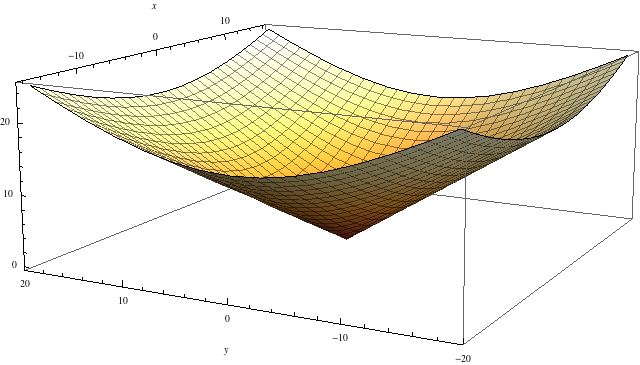
\includegraphics[width=0.8\textwidth]{img/Cono.png}  
		\caption{La función $f(x,y) = \sqrt{x^2+y^2}$} 
	\end{center}  
\end{figure}

\index{Cono}
Usando los conjuntos de nivel podemos reducir el problema de dibujar la superficie a encontrar las curvas que representan cada conjunto de nivel. Por ejemplo, tomando la función $f(x,y) = \sqrt{x^2+y^2}$. Si $c<0$, $N_c = \emptyset$. Si $c = 0$ entonces $N_0 = (0,0)$, y si $c>0$ entonces cada conjunto $N_c$ es una circunferencia de radio $c$ centrada en el origen.

Para ensamblar todos los conjuntos hacemos una sección vertical, por ejemplo usando el plano $x=0$. En este caso, la función que sale es $z=\abs{y}$, por lo que la superficie es un cono.

\begin{figure}[hbtp]    
	\begin{center} 
		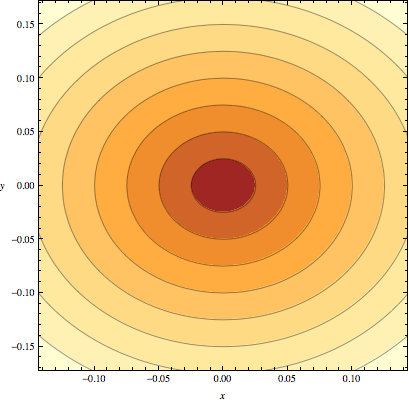
\includegraphics[width=0.7\textwidth]{img/ConoContorno.png} 
		\caption{Las líneas de contorno de $f$} 
	\end{center}  
\end{figure}

\begin{figure}[hbtp]    
	\begin{center} 
		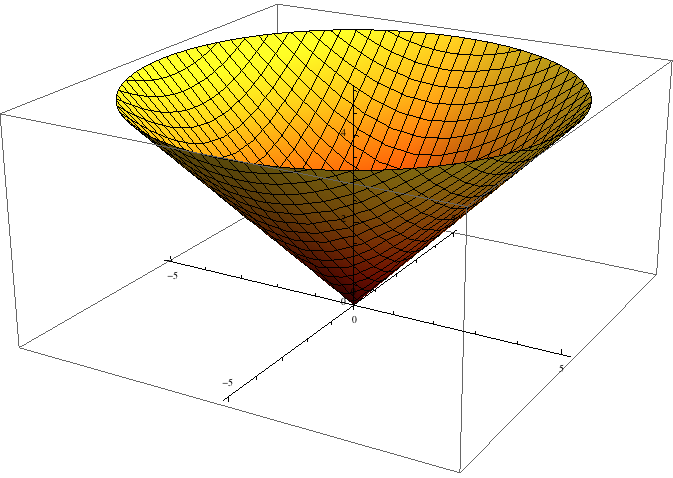
\includegraphics[width=0.8\textwidth]{img/Cono2.png}  
		\caption{La función dibujada} 
	\end{center}  
\end{figure}

\subsubsection{Funciones de $\real^3$ a $\real$}

En las funciones de tres variables también podemos usar los conjuntos de nivel como superficies, de forma que podemos hacernos una idea de cómo sería la función en $\real^4$.

\subsection{Límites}

\begin{defn}[Límite]Sea $\appl{f}{\real^N}{\real^M}$. Entonces

\[ \lim_{\vx\to\va} f(\vx) = \vec{L} \dimplies \forall \epsilon >0\; , \exists \delta > 0 \tq 0<\md{\vx-\va} < \delta \implies \md{f(\vx ) - \vec{L}} \]

\end{defn}


Las propiedades de los límites en varias dimensiones son las siguientes:

\begin{itemize}
\item El límite es único.
\item Sea $f=(f_1, f_2,\cdots, f_M)$ y $\vec{L} = (L_1, \cdots, L_M)$. Entonces, $\lim_{\vx\to\va} f(\vx) = \vec{L} \dimplies \lim_{\vx\to\va} f_j(\vx) = L_j\;\; , j=1\cdots M$.
\item $\lim (f+g) = \lim f +\lim g$.
\item $\lim \lambda f = \lambda \lim f$.
\item $\lim \frac{f}{g} = \frac{\lim f}{\lim g}$ si $\lim g \neq 0$.
\item Si en un entorno de $\va$ $f\leq g$ entonces $\lim f \leq \lim g$.
\end{itemize}

\subsubsection{Resolución de indeterminaciones}

\textbf{Indeterminación $0/0$:} Tomemos el siguiente límite.

\[ \lim_{(x,y)\to(0,0)} \frac{x^4}{\sqrt{x^2+y^2}} \]

Primero tomamos límites a lo largo de rectas $y=kx$. El límite se convierte entonces en un límite de una sola variable:

\[\lim_{x\to 0} \frac{x^4}{\sqrt{x^2+(kx)^2}} = \lim_{x\to 0} \frac{x^4}{\sqrt{x^2(1+k^2)}} = \lim_{x\to 0} \frac{x^4}{\abs{x}\sqrt{1+k^2}} = \lim_{x\to 0} \frac{\abs{x}^3}{\sqrt{1+k^2}} = 0\; \forall k\]

Con esto logramos una conjetura del límite, que podemos probar o bien con la definición de límite o bien con el criterio de comparación. Como podemos acotar la expresión

\[ 0 \leq \frac{x^2x^2}{\sqrt{x^2+y^2}} \leq \frac{x^2(x^2+y^2)}{\sqrt{x^2+y^2}} = x^2\sqrt{x^2+y^2} \]

y es obvio que $x^2\sqrt{x^2+y^2}$ tiende a $0$ cuando $x\to 0$, entonces por criterio de comparación (lema del sándwich), nos queda que

\[\lim_{(x,y)\to(a,b)}\frac{x^4}{\sqrt{x^2+y^2}} = 0 \]

Sin embargo, que el límite de cualquier recta sea 0 no implica que el límite sea ese número. Por ejemplo, sea $f$ la siguiente función:

\[ f (x,y) = \left\lbrace \begin{matrix} 1\; si\; y=x^2 \\ 0 \; si \; y\neq x^2  \end{matrix}\right. \]

El límite a lo largo de cualquier recta en el origen es $0$. Sin embargo, si me acerco al origen a través de la parábola $y=x^2$ es límite es $1$. Por lo tanto, el límite no existe.

\subsection{Continuidad}

\begin{defn}[Función\IS continua] Una función $f$ es continua en $\va$ si y sólo si $f(\va) = \lim_{\vx\to\va} f(\vx)$. Es decir:

\[ \forall \epsilon > 0\; , \exists \delta > 0 \tq \md{\vx-\va} < \delta \implies \md{f(\vx)-f(\va)} \]
\end{defn}

\begin{theorem}[Caracterización en términos de sucesiones]
$F$ es continua en $\va$ si y sólo si para toda sucesión $\{\vx_n\}$ con $\lim_{n\to\infty} \vx_n = \va$, se tiene que $\lim_{n\to\infty} F(\vx_n) = F(\va)$.
\end{theorem}

Las funciones continuas cumplen las mismas propiedades algebraicas que los límites. Además, la función de cada una de las coordenadas de una función continua también es continua.

\begin{theorem}[Continuidad de la composición]
Si $F$ es continua en $\va$ y $G$ es continua en $F(\va)$, entonces $G\circ F$ es continua en $\va$
\end{theorem}

\begin{defn}[Función\IS inversa]
Sea $\appl{F}{\real^N}{\real^M}$, y $A\subset \real^M$, definimos la función inversa: \[\inv{F}(A) = \{ \vx\in\real^N\tq F(\vx) \in A \}\]
\end{defn}

\begin{theorem}
$F$ es continua si y sólo si para todo conjunto abierto $A$ $\inv{F}(A)$ es abierto.
\end{theorem}

\begin{theorem}
$F$ es continua si y sólo si para todo conjunto cerrado $B$ $\inv{F}(B)$ es cerrado.
\end{theorem}

\section{Diferenciabilidad de funciones $\real^N \mapsto \real^M$}

\begin{defn}[Derivada\IS parcial]
La derivada parcial de una función es la derivada con respecto a una única variable. Notación: 

\[ \frac{\partial F}{\partial x} \]
\end{defn}


El problema de la derivabilidad en varias variables es que no podemos buscar la aproximación igual que en una variable. Buscamos entonces una aproximación lineal, donde

\[ F(\vx) = F(\va) +DF(\vx) + \epsilon \]

Donde $\epsilon$ es el error que cumple que \[\lim_{\vx\to\va} \frac{\epsilon}{\md{\vx-\va}} =0\]. $D$ es el \textbf{diferencial}, que depende de la función.

\begin{defn}[Diferencial]
Sea $\appl{F}{\real^N}{\real^M}$, tal que $F(x_0,\cdots,x_n) = (y_0, \cdots, y_m)$. Entonces, el diferencial es una matriz de dimensión $M\x N$ que se define como
 

\[ DF = \left( \begin{matrix} \dpa{y_1}{x_1} & \cdots &\frac{y_1}{x_n} \\
\vdots & \ddots & \vdots \\
\dpa{y_m}{x_1} & \cdots & \dpa{y_m}{x_n} \end{matrix}\right) \]

El diferencial cumple la siguiente identidad: 

\[ \lim_{\vx\to\va} \frac{\md{(F(\vx) - F(\va)) - DF(\va)(\vx-\va)}}{\md{\vx-\va}} = 0 \]
\end{defn}

\begin{theorem}
Si $F$ es diferenciable en $\va$, entonces $F$ es continua en $\va$.
\end{theorem}

\begin{theorem}
Si $F$ es diferenciable, entonces existen todas las derivadas parciales. Atención: el recíproco no es cierto.
\end{theorem}

\begin{theorem}
Si existen todas las derivadas parciales y además son continuas, entonces la función es diferenciable.
\end{theorem}

\begin{remark}
Si las parciales no son continuas pueden darse los dos casos, que sea o no sea diferenciable.
\end{remark}

\subsection{Operaciones con derivadas}

Se aplican las mismas reglas que en una dimensión.

\subsubsection{Regla de la cadena}

Tenemos dos funciones, $\appl{F}{\real^M}{\real^K}$ y $\appl{G}{\real^N}{\real^M}$, y consideramos su composición $H=\appl{F\circ G}{\real^N}{\real^K}$.

\begin{theorem}
Si $G$ es diferenciable en $\va$ y $F$ diferenciable en $G(\va)$ entonces $H$ es diferenciable en $\va$. Además:

\[DH (\va) = DF(G(\va))\cdot DG(\va) \]
\end{theorem}

\begin{theorem}
Sea $A$ una matriz y $\vx$ un vector. Se tiene entonces que 

\[ A\vx \leq C\md{\vx} \]

donde $C$ es una constante. Esto es útil para probar la regla de la cadena.
\end{theorem}

Se puede abreviar la obtención de cada derivada parcial del diferencial de la siguiente forma:

\[ \dpa{H_a}{x_b} = \sum_{i=0}^M\dpa{H_a}{y_i}\cdot \dpa{y_i}{x_b} \]


donde $y_1$ es cada una de las variables de $F$.

\subsection{Derivadas direccionales}

La derivada direccional nos indica cómo crece la función en una dirección determinada por un vector. La definición estricta viene a continuación:

\begin{defn}[Derivada\IS direccional]
Dada una función $\appl{F}{\real^N}{\real}$ y un vector unitario $\vu$, llamamos $D_{\vu} F(\va)$ a la derivada de $F$ en el punto $\va$ en la dirección $\vu$. Si llamamos $g(t) = F(\va + t\vu)$, entonces

\[ D_{\vu} F(\va) \equiv g'(0) = \left.\deriv{F(\va + t\vu)}{t}\right|_{t=0} \]
\end{defn}

\begin{theorem}
Si $F$ es derivable, entonces $D_{\vu} F(\va) = \pesc{\nabla F(\va), \vu}$.
\end{theorem}

\subsection{Gradiente}
\begin{defn}[Gradiente]
Sea $\appl{F}{\real^N}{\real}$. Entonces, se define el gradiente como 

\[ \nabla F \in \real^N = \left(\dpa{F}{x_1},\cdots,\dpa{F}{x_n}\right) \]
\end{defn}

El gradiente es un caso especial de la matriz diferencial, y cumple estas dos propiedades:

\begin{enumerate}
\item El gradiente vive en el mismo espacio que los conjuntos de nivel, no en el de la imagen.
\item $\nabla F$ es la dirección de máximo crecimiento de la función.
\end{enumerate}

\subsubsection{Plano tangente a través del gradiente}
\index{Plano!tangente}
Además, el gradiente permite calcular el plano tangente a una superficie, tanto en superficies dadas como conjuntos de nivel $F(x,y,z) = C$ como en superficies dadas como gráficas $z=f(x,y)$. 

Vamos con el primer caso: tomamos la superficie $S\equiv \{(x,y,z) \tq F(x,y,z) = C\}$, el punto $\va$ y la curva $\sigma (t)$ que cumple que $\sigma (t) \subset S \; \forall t$ y que $\sigma (0) = \va$.

Denomimamos $g(t) = F(\sigma(t)) = C$, por lo que $g'(t) =0$. En particular, tenemos que $\pesc{\nabla F (\va), \sigma ' (0)}= 0$. Dado que $\sigma$ es una curva arbitraria, obtenemos que $\nabla F (\va)$ es perpendicular a todos los vectores tangentes a la superficie. Por lo tanto, $\nabla F (\va)$ es perpendicular al plano tangente a $S$ en $\va$.

De esta forma, podemos definir el plano tangente según la siguiente ecuación:

\[ 0 =\pesc{\nabla F(\va),\vx -\va} \]

Vamos ahora con el segundo caso, donde $S\equiv \{z=f(x,y) \}$. Hay dos métodos posibles, el primero es usando el cálculo anterior tomando $F(x,y,z) = f(x,y) - z = 0$. De esta forma, nos quedaría que el plano tangente a $S$ en el punto $(a,b)$ tendría la siguiente ecuación:

\[ f(a,b) + \dpa{f}{x} (a,b) (x-a)+\dpa{f}{y}(a,b) (y-b) - z = 0 \]

También podemos obtenerlo directamente. Tomamos una curva con $x$ constante, esto es $\sigma_1(y) = (a,y, f(a,y))$, cuya derivada es $\sigma_1'=(0,1,\dpa{f}{y})$. Hacemos lo mismo con $y$ constante, quedándonos $\sigma_2 = (x, b, f(x,b))$ y $\sigma_2 ' = (1, 0, \dpa{f}{x})$. Así nos quedaría un vector $\vn$ perpendicular a $S$:

\[ \vn = \sigma_1'\x\sigma_2' = \left(\dpa{f}{x}, \dpa{f}{y}, -1\right) \]

y que es el mismo que habíamos obtenido con el anterior método.

\subsection{Derivadas paramétricas}

Una función paramétrica se da de la siguiente forma:

\[ \left\lbrace \begin{matrix}
x = x(t) \\ y = y(t)
\end{matrix}\right. \]

Si derivamos $x(t)$ y $y(t)$, tenemos el vector director de la recta tangente a la curva para un parámetro t. Además, tenemos que

\index{Derivada!paramétrica}
\[ \deriv{y}{x} = \deriv{y}{t} \cdot \deriv{t}{x} \]

\subsection{Derivadas de orden superior}

La derivada de orden superior consiste en derivar varias veces una función. Por ejemplo, si $f$ es una función:

\[ \dpa{}{x}\left(\dpa{f}{y}\right)  \]

consistiría en derivar primero $f$ con respecto de $y$ y después con respecto de $x$.

\begin{theorem}[Teorema de las derivadas cruzadas de Euler][Derivadas\IS cruzadas]
Sea $F\in C^2$, $\appl{F}{\real^N}{\real}$. Entonces

\[ \frac{∂^2 f}{∂x∂y} = \frac{∂^2 f}{∂y∂x} \]
\end{theorem}

\begin{proof}
Definimos $G(h,k) = F(x_0+h, y_0+k) - F(x_0+h, y_0) - F(x_0, y_0 +k) + F(x_0, y_0)$. $k$ es fijo y $h$ variable, y definimos $g(s) = F(s, y_0 + k) - F(s, y_0)$. Con esta notación, $G(h,k) = g(x_0+h) - g(x_0)$. Según el teorema del valor medio:

\[ G(h,k) = g'(\tilde{s})h \]

para algún $\tilde{s} \in [x_0, x_0+h]$. Derivando, tenemos que

\[ g'(s) = \frac{∂F}{∂x}(s, y_0+k) - \frac{∂F}{∂x} (s, y_0) \]

Definimos $H(t) = \frac{∂F}{∂x} (\tilde{s}, t)$. Entonces, tenemos que 

\[G(h,k) = H'(\tilde{t})kh \]

para algún  $\tilde{t} \in [y_0, y_0+k]$. Si derivamos, tenemos que 

\[ H'(t) = \frac{∂^2 F}{∂y∂x}(\tilde{s}, t) \]

Entonces, nos queda $G(h,k) = \frac{∂^2F}{∂y∂x}(\tilde{s}, \tilde{t}) h k$, es decir

\[\frac{∂^2F}{∂y∂x}(\tilde{s}, \tilde{t}) = \frac{G(h,k)}{hk} \]

Si tenemos en cuenta que cuando $h\to 0$ y $k\to 0$ $\tilde{s}$ y $\tilde{t}$ tienden a cero respectivamente, entonces

\[ \frac{∂^2F}{∂y∂x}(x_0, y_0) = \lim_{(h,k) \to (0,0)} \frac{G(h,k)}{hk} \] 

Si repitiésemos la misma prueba paso a paso pero en lugar de empezar tomando la devirada en $x$ la tomamos en $y$, obtendremos el mismo resultado.
\end{proof}

A partir del teorema, podemos obtener la matriz de derivadas segundas:

\begin{defn}[Matriz\IS Hessiana]
\[D^2f(a,b) = \left(\begin{matrix} \frac{\partial^2 f}{∂ x^2} (a,b) & \frac{\partial^2 f}{\partial x \partial y} (a,b) 
\\ \frac{\partial^2 f}{\partial y \partial x} (a,b) & \frac{\partial^2 f}{\partial y^2} (a,b) \end{matrix}\right) \]
\end{defn}

\subsection{Máximos y mínimos}

\begin{defn}[Máximo/mínimo\IS local] Sea $\appl{f}{\real^N}{\real}$. Diremos que $\vx_0 \in \real^N$ es un punto de máximo local si $\exists \epsilon > 0 \tq F(\vx_0) \geq F(\vx)\;\; \forall \vx \in B_{\epsilon} (\vx_0) $

La definición es análoga para el mínimo\end{defn}

\begin{remark} Por las propiedades del gradiente, si $F$ es diferenciable y $\vx_0$ es un máximo o mínimo local, entonces debe ser $\nabla F(\vx_0) = \vec{0}$.\end{remark}

\begin{defn}[Punto\IS crítico] $\vx \in \real^N$ es un punto crítico de $F$ si y sólo si $\nabla F(\vy) = \vec{0}$\end{defn}

No todos los puntos críticos son máximos o mínimos, así que tenemos que clasificarlos de alguna forma. Para ello, usamos el polinomio de Taylor de orden 2, de forma que 

\[
F(x,y) = F(x_0, y_0) + \pesc{\nabla F(x_0, y_0), (x-x_0, y-y_0)} +\]\[\frac{1}{2}(x-x_0, y-y_0)\left(\begin{matrix} \frac{\partial^2 f}{∂ x^2} (x_0,y_0) & \frac{\partial^2 f}{\partial x \partial y} (x_0,y_0) 
\\ \frac{\partial^2 f}{\partial y \partial x} (x_0,y_0) & \frac{\partial^2 f}{\partial y^2} (x_0,y_0) \end{matrix}\right) \left(\begin{matrix} x - x_0 \\ y - y_0 \end{matrix}\right) + \epsilon \]

Simplificando nos queda que:

\[F(\vx) = F(\vx_0) + \pesc{\nabla F(\vx_0), \vx - \vx_0} + \frac{1}{2}(\vx - \vx_0) D^2F(\vx_0) (\vx - \vx_o) ^T + \epsilon\]

Dado que el gradiente es 0, el punto clave es el signo de $\frac{1}{2}(\vx - \vx_0) D^2F(\vx_0) (\vx - \vx_o) ^T$. Para ello, usamos las siguientes definiciones del álgebra lineal.

\subsubsection{Resultados de álgebra lineal}
\index{Matriz!semidefinida positiva/negativa}
\index{Matriz!definida positiva/negativa}
\begin{defn}[Matriz semidefinida y definida positiva y negativa][]
\noindent\\ \indent
La matriz $A$ de dimensión $N\x N$ es semidefinida positiva si y sólo si $\vv A \vv^T \geq 0 \;\; \forall \vv \in \real^N$.

La matriz $A$ de dimensión $N\x N$ es definida positiva si y sólo si $\vv A \vv^T > 0 \;\; \forall \vv ≠0 \in \real^N$.

La matriz $A$ de dimensión $N\x N$ es semidefinida negativa si y sólo si $\vv A \vv^T \leq 0 \;\; \forall \vv \in \real^N$.

La matriz $A$ de dimensión $N\x N$ es definida negativa si y sólo si $\vv A \vv^T < 0 \;\; \forall \vv ≠0 \in \real^N$.
\end{defn}

\begin{theorem}
Si una matriz es simétrica, existe una base en la cual la matriz es diagonal.
\end{theorem}

\index{Autovalor}
\index{Autovector}
Sea $A$ una matriz $N\x N$. Entonces diremos que un vector $\vv ≠ \vec{0}$ es un autovector asociado al autovalor $\lambda\in \real$ si y sólo si $A\vv = \lambda\vv$. Dado que podemos escribir

\[ A = \left(\begin{matrix}
a & b \\ c &  d
\end{matrix}\right)\;\;\;\; \vv = \left(\begin{matrix}
x\\ y
\end{matrix}\right) \], entonces tenemos que $A\vv = \lambda \vv$ si y sólo si

\[ \left\lbrace\begin{matrix}ax+by=\lambda x \\ cx+dy = \lambda y \end{matrix}\right. \]

Es decir, la autorrecta $\begin{pmatrix}x \\ y \end{pmatrix}$ es una solución no trivial del sistema anterior. Sin embargo, para que haya soluciones no triviales el determinante de la matriz $\begin{pmatrix}a-\lambda & b \\ c & d - \lambda\end{pmatrix}$ debe ser 0.

Por lo tanto, los autovalores son las soluciones de la ecuación $det(A-\lambda I) = 0$, siendo $I$ la matriz identidad.

\begin{theorem}
Si un conjunto de autovectores es una base, entonces la matriz $A$ expresada respecto a esa base pasa a ser diagonal, y los elementos de la diagonal son los autovalores. 

Si dos autovalores son distintos, los autovectores asociados son distintos.

Si A es simétrica, entonces el conjunto de autovectores es una base.
\end{theorem}

Volvemos ahora al cálculo.

\begin{theorem}[Clasificación de puntos críticos][]
Sea $\appl{F}{\real^N}{\real}$, $F\in C^2$ (con dos derivadas continuas), y sea $\vx_0$ un punto crítico. Entonces

\begin{enumerate}
\index{Máximo/mínimo!local}
\index{Punto!de silla}
\index{Punto!crítico degenerado}

\item Si \textbf{todos} los autovalores de $D^2F(\vx_0)$ son \textbf{mayores que cero}, entonces $D^2F(\vx_0)$ es definida positiva y $\vx_0$ es un \textbf{mínimo local}.
\item Si \textbf{todos} los autovalores de $D^2F(\vx_0)$ son \textbf{menores que cero}, entonces $D^2F(\vx_0)$ es definida negativa y $\vx_0$ es un \textbf{máximo local}.
\item Si \textbf{algunos} autovalores son \textbf{mayores que cero} y otros son \textbf{menores que cero}, entonces $\vx_0$ es un \textbf{punto de silla.}
\item Si algún autovalor \textbf{es 0}, y el resto son mayores o menores que cero, entonces $\vx_0$ es un \textbf{punto crítico degenerado}.
\end{enumerate}
\end{theorem}

\subsubsection{Ejemplos}

Tomamos $F(x,y) = x^2 + y^2 +xy$. Obtenemos los puntos críticos, es decir, los puntos en los que $\nabla F(x,y) = (0,0)$. El punto resultante es $(0,0)$. Estudiamos el tipo de punto crítico. Para ello, calculamos la matriz hessiana en ese punto:

\[ D^2F(0,0) = \begin{pmatrix}2&1\\1&2\end{pmatrix}\]. 

Los autovalores son las soluciones de

\[ 0 = det\left(\begin{pmatrix}2&1\\1&2\end{pmatrix} - \lambda \begin{pmatrix}1&0\\0&1\end{pmatrix}\right) = det\begin{pmatrix}2-\lambda & 1 \\ 1 & 2-\lambda\end{pmatrix} = (2-\lambda)^2  - 1\]

Por lo tanto, $\lambda$ es $3$ o $1$. Dado que ambos autovalores son mayores que 0, entonces $D^2F$ es definida positiva y $(0,0)$ es un mínimo local.

\subsection{Máximos y mínimos absolutos}

\begin{defn}[Máximo y mínimo absoluto][] Sea $\appl{F}{\real^N}{\real}$ y $A\subset \real^N$. $\vx_m$ es un máximo absoluto de $F$ en $A$ si y sólo si $F(\vx_m) ≥ F(\vx)\;\; \forall \vx \in A$. La definición es análoga para el mínimo.
\end{defn}

\begin{theorem}[Teorema de compacidad]
Tenemos un conjunto $K\subset \real^N$ compacto (cerrado y acotado). Supongamos la sucesión $\{\vx_n\}_{n\in\nat}\subset K$. Entonces podemos encontrar al menos una subsucesión $\{\vx_{n_j}\}_{j\in\nat} \subset \{\vx_n\}_{n\in\nat}$ tal que $\{\vx_{n_j}\}$ es convergente.
\end{theorem}

\begin{proof}
Trabajamos en dimensión 2, pero la demostración es análoga.
Como $K$ es compacto, podemos encontrar un cuadrado $Q_0$ de lado $L$ que encierre completamente a $K$. Divido $Q_0$ en $2^2$ cuadrados de lado $L/2$.  En alguno de ellos hay infinitos términos de la sucesión: lo llamamos $Q_1$ y me quedo con uno de los términos de la sucesión, al que llamamos $x_1$. Volvemos a dividir este cuadrado en cuatro cuadrados, elegimos uno que tenga infinitos términos de la sucesión y seleccionamos un elemento de la sucesión dentro al que llamamos $x_2$. Repetimos esto muchas veces, de forma que cada término $x_n$ está encerrado en el cuadrado $Q_n$ de lado $\frac{L}{2^n}$. 

Si $k,l > n$, entonces es claro que $\md{\vx_k-\vx_l}$ es menor o igual que la diagonal de $Q_n$, que es $\frac{L}{2^n}\sqrt{2}$, que tiende a cero cuando $n\to\infty$. Por el criterio de Cauchy, entonces esta sucesión es convergente, y como $K$ es cerrado el límite pertence a $K$.
\end{proof}

\begin{theorem}
Sea $K\subset \real^N$ compacto y $\appl{F}{\real^N}{\real}$, continua en $K$. Entonces, $F$ alcanza su máximo y mínimo absolutos en $K$.
\end{theorem}

\begin{proof}

Como $F$ es acotada, existe $\alpha = \sup \{ F(x) \tq x \in K\}$. Existe entonces una sucesión $\{x_n\}$ tal que si $n\to \infty$ entonces $F(x_n)\to \alpha$. 
Sabemos que existe $\{x_n\}\subset K$, por lo que existe una subsucesión$\{x_{n_j}\}$ convergente tal que $x_{n_j} \to x_0 \in K$

Como $F$ es continua, $F(x_{n_k})\to F(x_0)$, es decir $F(x_{n_j}) \to \alpha$, por lo tanto el supremo es el máximo.
\end{proof}

\subsubsection{Ejemplos}

La función a estudiar es $F(x,y) = x^2-y^2$ en la bola $\omega = \{ x^2 + y ^2 ≥ 1\}$. Es diferenciable en todo $\real$ porque es un poliniomio. 

Calculamos el diferencial y vemos qué ocurre cuando es 0 \[\nabla F = (2x, -2y) = (0,0) \implies (x,y) = (0,0)\]

Operando, vemos que el punto $(0,0)$ es un punto de silla. Ahora sólo queda ver el comportamiento en la frontera $C$, cuando $x^2+y^2 = 1$. $F$ restringida a $C$ quedaría de la siguiente forma:

\[ F(\cos t, \sin t) = \cos^2 t - \sin^2 t = \cos 2t\]

El coseno tiene máximos cuando $t=0$ y $t=\pi$, y mínimos cuando $t=\pi /2$ y $t=3\pi /2$. Es decir, tiene máximos absolutos en los puntos $(1,0),\;(-1,0)$ y mínimos absolutos en $(0, -1)$, $(0, 1)$. 

\begin{theorem}[Multiplicadores de Lagrange]
Tenemos una función $\appl{F}{\real^2}{\real}$ y una restricción $G(x_1,\cdots,x_n) = k$, resolvemos el siguiente sistema:

\begin{align*}
\nabla F &= \lambda \nabla G \\
G &= k
\end{align*} 

\end{theorem}

\section{Funciones $\real^N \mapsto \real^{>1}$}

\subsection{Curvas parametrizadas}
\subsubsection{Ejemplos}

\index{Cicloide}
La cicloide es un ejemplo de curva parametrizada en dos dimensiones, con la siguiente función:

\[ \sigma(t) = (t - \sin t, 1 - \cos t) \]

\begin{figure}[hbtp]    
	\begin{center} 
		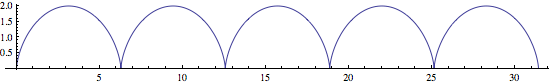
\includegraphics[width=0.8\textwidth]{img/Cicloide.png}  
		\caption{El cicloide evaluado desde 0 hasta $10 \pi$} 
	\end{center}  
\end{figure}

\subsubsection{Cálculo recta tangente}
\index{Recta!tangente}
Sea $\sigma (t) = (x_1 (t),x_2(t), x_3(t))$ una curva diferenciable. Hay dos casos posibles para formar la recta tangente:

Si $ (x_1' (t_0),x_2'(t_0), x_3'(t_0))≠ (0,0,0)$, entonces la recta tangente es la siguiente:

\[ \begin{pmatrix} x \\ y \\ z \end{pmatrix} = \begin{pmatrix}{x_1(t_0)} \\ {x_2(t_0)} \\ {x_3(t_0)}\end{pmatrix} + \lambda \begin{pmatrix}{x_1'(t_0)} \\ {x_2'(t_0)} \\ {x_3'(t_0)}\end{pmatrix} \]

Si, por el contrario, $\sigma'(t_0) = \vec{0}$, entonces normalizamos la derivada y hallamos el límite cuando $t\to t_0$:

\[ \lim_{t\to t_0} \frac{\sigma'(t)}{\md{\sigma'(t)}} \]

Si este límite existe, nos dará la dirección de la recta tangente. Si no existe, no hay recta tangente.

\paragraph{Ejemplos}
\subparagraph{Cicloide}

La función de la cicloide es $\sigma(t) = (t - \sin t, 1 - \cos t),\; t\in \real$. Cuando $t=0$, $\sigma'(0) = (0,0)$. Normalizamos entonces la derivada y nos queda que 

\[ \frac{\sigma'(t)}{\md{\sigma'(t)}} = \frac{1}{\sqrt{2}\sqrt{1 - \cos t}} (1 - \cos t, \sin t) \]

Tomamos el límite cuando $t\to 0$. La primera componente queda $0$, la segunda es más compleja:

\[ \frac{\sin t}{\sqrt{2}\sqrt{1 - \cos t}}\frac{ \sqrt{1 + \cos t}}{ \sqrt{1 + \cos t}} = \frac{\sin t \sqrt{1 + \cos t}}{\sqrt{2} \sqrt{\sin^2 t}} = \frac{\sqrt{1 + \cos t}}{\sqrt{2}} \frac{\sin t}{|\sin t |} \]

Esto tiende a $1$ cuando nos aproximamos por la derecha, y $-1$ cuando nos acercamos por la izquierda. No hay por lo tanto recta tangente.

\subsubsection{Cálculo de longitudes}
\label{refLong}
Tenemos una curva $\appl{\sigma}{[a,b]}{\real^N}$ de la que queremos buscar la longitud. Trabajamos en dimensión $N=3$ para simplificar, pero el resultado es generalizable. Dividimos el segmento en varios puntos $t_0, t_1, \cdots, t_n$. La longitud de un segmento que va del punto $t_i$ a $t_{i+1}$ es

\[ l = \sqrt{(x(t_{i+1}) - x(t_i) )^2 + (y(t_{i+1}) - y(t_i) )^2 + (y(t_{i+1}) - x(t_i) )^2} \]

Según el teorema del valor medio, si $s_i \in [t_i, t_{i+1}]$ entonces

\[ l = \sqrt{(x'(s_i)(t_{i+1}-t_i))^2+(y'(s_i)(t_{i+1}-t_i))^2+(z'(s_i)(t_{i+1}-t_i))^2} = (t_{i+1}-t_i)F(s_i) \]

donde \footnote{ En realidad, los $s_i$ no tienen por qué ser iguales para todas las coordenadas. Sin embargo, esto no afecta a la demostración, ya que cuando el intervalo se hace muy pequeño los puntos medios coinciden. }

\[ F(s_1) = \sqrt{(x'(s_i))^2+(y'(s_i))^2+(z'(s_i))^2} \]

Entonces, la longitud $L$ del segmento es 

\[ L = \lim_{n\to\infty} \sum = \int_a^b\md{\sigma'(t)}dt\]

\begin{theorem}[Longitud de arco][Integral!de línea]
Dada un curva parametrizada $\appl{\sigma}{\Omega\subset\real}{\real^N}$, la longitud de arco entre dos puntos $a, b\in \Omega$ es 

\[ \int_a^b\md{\sigma'(t)}dt \]
\end{theorem}

\paragraph{Ejemplos}
\subparagraph{Circunferencia}
Si $\sigma(\theta) = (R\cos\theta, R\sin\theta),\; \theta \in [0, 2\pi]$, entonces 

\[ \sigma'(\theta) = (-R\sin\theta, R\cos\theta) \]
\[ \md{\sigma'(\theta)} = \sqrt{R^2 \sin^2\theta + R^2 \cos^2\theta} = R \]

Integramos

\[ \int_0^{2\pi} \md{\sigma'(\theta)}d\theta = \int_0^{2\pi} Rd\theta = 2\pi R \]

\subparagraph{Cardioide}
\index{Cardioide}
La ecuación es $\sigma(t) = ((1+\cos t)\cos t, (1+\cos t)\sin t)$, la derivada es $\sigma'(t) = (-\sin t - \sin 2t,\cos t + \cos 2t)$. Calculamos el módulo:

\[ \md{\sigma'(t)} = \sqrt{2}\sqrt{1+\cos t} \]

Integramos:

\[ L = \int_0^{2\pi}\sqrt{2}\sqrt{1+\cos t} \;dt = 8 \]

\subsection{Superficies parametrizadas}
\subsubsection{Ejemplos}

\index{Helicoide}\label{Helicoide}
El \textbf{helicoide} es una función $\Phi$ de dos variables, que crea una superficie helicoidal (escalera de caracol) en el espacio, tal que 

\begin{align*} \appl{\Phi}{\real^2 &}{\real^3} \\
 (s,t) &\longmapsto \Phi(s,t) = (s\cos t, s\sin t, t) \end{align*}
 
\begin{figure}[hbtp]    
	\begin{center} 
		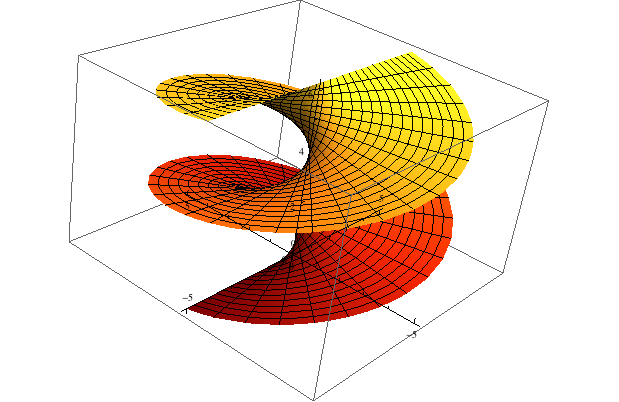
\includegraphics[width=0.8\textwidth]{img/Helicoide.png}  
		\caption{El helicoide} 
	\end{center}  
\end{figure}

En general, una superficie parametrizada es una aplicación $\Phi$ de la siguiente forma:

\begin{align*} \appl{\Phi}{\Omega \subset \real^2 &}{\real^3} \\
 (s,t) &\longmapsto \Phi(s,t) = (x(s,t), y(s,t), z(y,t)) \end{align*}

\index{Paraboloide}
Por ejemplo, el \textbf{paraboloide} se puede definir como una superficie parametrizada \[\Phi(x,y) = (x,y,x^2+y^2)\].

\index{Cilindro}
Otro ejemplo es el \textbf{cilindro} de radio 2. Para parametrizarlo, usamos coordenadas polares de la siguiente forma:

\[ \Phi(t,z) = (2\cos t, 2\sin t, z)\;\;t\in [0, 2\pi],\;\; z\in \real \]

\index{Esfera}
Si queremos hacer la \textbf{esfera} de radio $R$, en la parametrización usamos dos parámetros (longitud y latitud)

\[ \Phi(\theta, \phi) = (R\sin\phi\cos\theta, R\sin\phi\sin\theta, R\cos\phi)\;\; \theta\in[0,2\pi],\;\;\phi\in[0, \pi] \]

\index{Toro}
El \textbf{toro} (una especie de flotador) se produce al girar una circunferencia de radio $R_1$ en el plano $XZ$ con el centro sobre el eje $X$ a $R_2$ del origen alrededor del eje $Z$.

\[ \Phi(\theta, \phi) = ((R_2+R_1\cos\phi)\cos\theta,(R_2+R_1\cos\phi)\sin \theta,R1\sin \phi)\;\; \theta, \phi \in [0, 2\pi] \]

\begin{figure}[hbtp]    
	\begin{center} 
		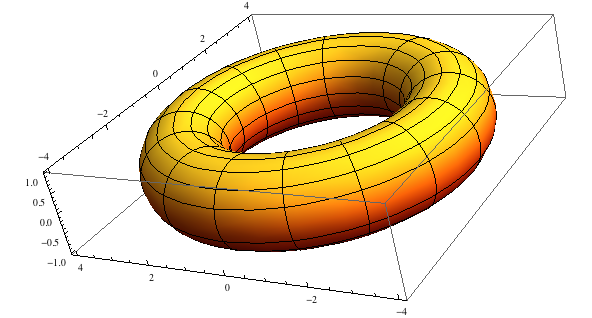
\includegraphics[width=0.8\textwidth]{img/Toro.png}  
		\caption{Toro} 
	\end{center}  
\end{figure}

\subsubsection{Parametrización de superficies de revolución}
\index{Superficie!de revolución}

Dada una función $\appl{f}{\real}{\real}$, la superficie de revolución que surge al rotar esta función sobre el eje z es la siguiente

\begin{align*} z(r,\theta) &= f(r) \\
x(r,\theta) &= r \cos \theta \\
y(r,\theta) &= r \sin \theta \end{align*} 

\subsubsection{Coordenadas cilíndricas}
\index{Coordenadas!cilíndricas}
Dado un punto $P$, sus coordenadas cartesianas son $(x,y,z)$. Entonces, sus coordenadas cartesianas son $(r,\theta, z)$, donde $r\in [0,\infty)$, $\theta \in [0,2\pi]$ y $z\in \real$. La correspondencia es la siguiente:

\begin{align*}
x &=r \cos \theta \\
y &= r \sin \theta \\
z &= z
\end{align*}

Geométricamente, $z$ es la altura de $P$. Haciendo la proyección del punto sobre el plano $xy$, $r$ es la distancia de la proyección al origen y $\theta$ el ángulo del eje $X$ con la recta que une el origen y la proyección del punto.

\subsubsection{Coordenadas esféricas}
\index{Coordenadas!esféricas}
Las coordenadas esféricas de un punto $P$ son $(\rho, \theta, \phi)$, donde $\rho \in [0, \infty)$, $\theta\in [0, 2\pi]$, $\phi \in [0, \pi]$. La correspondencia con coordenadas cartesianas es

\begin{align*}
x&=\rho \cos \theta \sin \phi \\
y&= \rho \sin \theta \sin \phi \\
z &= \rho \cos \theta
\end{align*}

Geométricamente, $\rho$ es la distancia de $P$ al origen, $\theta$ es el ángulo que forman el eje $X$ y la recta que une $P$ y el origen, y $\phi$ es el ángulo que forman el eje $Z$ y esa misma recta.

\subsubsection{Usos de coordenadas esféricas y cilíndricas}

En las coordenadas cilíndricas, si mantenemos constante un parámetro y variamos los otros dos obtenemos varias superficies:

\begin{itemize}
\item Si $r$ constante, tenemos un cilindro. \index{Cilindro}
\item Si $\theta$ constante, tenemos un semiplano. \index{Semiplano}
\item Si $z$ constante, tenemos un plano horizontal. \index{Plano}
\end{itemize}

Lo mismo ocurre con las coordenadas esféricas:

\begin{itemize}
\item Si $\rho$ constante, tenemos una esfera. \index{Esfera}
\item Si $\theta$ constante, tenemos un semiplano.\index{Semiplano}
\item Si $\phi$ constante, tenemos un cono. \index{Cono}
\end{itemize}

\subsubsection{Cálculo del plano tangente}
\index{Plano!tangente}
Tenemos una superficie $\appl{\Phi}{\Omega\subset\real^2}{\real^3}$ de la que queremos calcular el plano tangente en un punto $P = (x(u_0, v_0),y(u_0, v_0),z(u_0, v_0))$. Si mantenemos fijo $v$ y variamos $u$ (nos movemos sobre una recta), tenemos que 

\[ \Phi(u, v_0) = \sigma_1(u) = (x(u, v_0),y(u, v_0),z(u, v_0)) \]
cuyo vector tangente es $\nabla \sigma_1'(u_0) \equiv T_u (u_0, v_0)$. De la misma forma obtenemos el vector tangente en la dirección $v$ al que denotamos $T_v(u_0, v_0)$. Calculamos entonces el vector $\vv = T_u(u_0, v_0)\x T_v(u_0, v_0)$ que es normal al plano, y a partir del cual obtenemos la ecuación del plano.


\paragraph{Ejemplos}
\index{Helicoide}
\subparagraph{Helicoide} La ecuación  del helicoide es $\Phi(s,t) = (s\cos t, s\sin t, t)$. Calculamos los vectores tangentes:

\[ T_s = \nabla \Phi(s, t_0) = (\cos t_0, \sin t_0, 0) \]
\[ T_t = \nabla \Phi(s_0, t) = (-s_0\sin t_0, s_0 \cos t_0, 1) \]

Calculamos el vector normal

\[ \vec{n} = T_s \x T_t = \cdots = (\sin t_0, -\cos t_0, s_0) \]

La ecuación del plano es entonces

\[ R\equiv \pesc{(x,y,z) - P}{\vec{n}} = 0 \]

\subsection{Campos vectoriales}
Los campos vectoriales son funciones $\appl{F}{\real^N}{\real^N}$, en el que a cada punto se le asigna un vector.
\index{Campo!vectorial}

\begin{defn}[Campo gradiente][Campo\IS gradiente o conservativo]
Diremos que $F$ es un campo gradiente o conservativo si $\exists \appl{V}{\real^N}{\real}$ tal que $F=\nabla V$.
\end{defn}

\begin{defn}[Divergencia]
En un campo vectorial, la divergencia mide el cambio de volumen y existencia de fuentes o sumideros. Si la divergencia es 0, tenemos un "fluido" incompresible.

\[ \textrm{div}\;F = \frac{∂F_1}{∂x_1} + \cdots + \frac{∂F_n}{∂x_n} \]
\end{defn}

\begin{defn}[Rotacional]
El rotacional mide el giro interno de las partículas en un campo, que se puede expresar como \footnote{En realidad, $\nabla$ no es un vector y esto es sólo una regla mnemotécnica}

\[ \textrm{rot}\;F = \nabla \x \vf \]

Si el rotacional es distinto de cero, significa que ha habido choques internos de las partículas y por lo tanto ha habido pérdida de energía.
\end{defn}

\begin{theorem}
Supongamos que $F\in C^1$ es un campo gradiente. Entonces, $\rot F = \vec{0}$. El recíproco también es cierto.
\end{theorem}

\begin{proof}
Al ser un campo gradiente, $F=\nabla V$. En cada una de las coordenadas tenemos $\frac{∂}{∂x_a}\left(\frac{∂V}{∂x_b}\right) - \frac{∂}{∂x_b}\left(\frac{∂V}{∂x_a}\right)$, que según el teorema de las derivadas cruzadas de Euler es 0.
\end{proof}

\begin{defn}[Laplaciano]
El laplaciano es la divergencia de un campo gradiente $F$. Si $F = \nabla V$, entonces

\[\dv F = \nabla \cdot \nabla V = \frac{∂^2V}{∂x_1^2} + \cdots + \frac{∂^2V}{∂x_n^2} = \nabla^2 V \]
\end{defn}

\section{Integración}

Tomemos una función en dimensión dos, $\appl{f}{\real^2}{\real}$ definida en un rectángulo $[a,b]\x[c,d]$. Su gráfica será una determinada superficie. El problema de la integración consiste en hallar el volumen encerrado bajo esa superficie.

El punto de partida es similar al método en dimensión 1: sabemos calcular el volumen de prismas rectangulares. Lo que haremos será particionar el rectángulo en varios subrectángulos, a cada uno de los cuales le corresponde un prisma que aproxima por debajo y otro por encima. A medida que aumentamos el número de subrectángulos, los volúmenes se aproximan y si existe el límite, será el volumen que buscamos.

\paragraph{Procedimiento}

Lo primero que hacemos entonces es hacer la partición del rectángulo inicial $[a,b]\x[c,d]$. Hacemos particiones del intervalo $[a,b]$ en subintervalos $[x_i, x_{i+1}]$ y del $[c,d]$ en subintervalos $[y_k, y_{k+1}]$. Entonces, tenemos los subrectángulos $R_{ik}=[x_i, x_{i+1}]\x[y_i, y_{i+1}]$, donde $i=1,\cdots,n$ y $k=1, \cdots, m$.

A partir de esto, aproximamos por prismas rectangulares rectos. A cada $R_{ik}$ le corresponde un mínimo $m_{ik} = \inf \{f(x,y)\tq (x,y)\in R_{ik}\}$ y análogamente un máximo $M_{ik}$.

Ahora hacemos la aproximación por arriba y por abajo. Sea $\mathcal{P}$ la partición hecha al comienzo, definimos la suma superior $U$ como

\[ U(f,\mathcal{P}) = \sum_{i,k} M_{ik} \cdot \text{Área}(R_{ik}) \]

y análogamente definimos la suma inferior $L(f,\mathcal{P})$.

A partir de aquí, tomamos los límites. Tomamos $\alpha = \inf\{U( f, \mathcal{P})\tq \mathcal{P} \text{ partición}\}$ y $\beta = \sup\{L(f, \mathcal{P})\tq \mathcal{P} \text{ partición}\}$. Por lo tanto, la función es integrable si $\alpha=\beta$. La notación es la siguiente:

\[ {\int\int}_{[a,b]\x[c,d]}f(x,y)dxdy=\alpha = \beta \]

\begin{theorem}[Función integrable]\index{Función!integrable}
$F$ es integrable si y sólo si $\forall \epsilon > 0$ podemos encontrar una partición $\mathcal{P}_\epsilon$ tal que $U(f,\mathcal{P}_\epsilon) - L(f,\mathcal{P}_\epsilon) < \epsilon$.
\end{theorem}

\begin{theorem}
Si $F$ es acotada y continua, entonces es integrable.
\end{theorem}

\paragraph{Ejemplos de funciones no integrables} 

\[ f(x,y) \left\{ \begin{matrix}
1 &\text{ si } x\in\cplex \y y\in\cplex \\
0&\text{ en otro caso}
\end{matrix}\right.\]

\begin{defn}[Conjunto\IS de área cero]
Un $A\subset \real^2$ tiene área cero si y sólo si $\forall\epsilon > 0$ lo podemos recubrir por una familia finita de rectángulos $R_1,\cdots,R_k$ tales $\text{Área}(R_1) +\cdots + \text{Área}(R_k) ≤ \epsilon$.

Son conjuntos de área cero los puntos aislados, rectas y curvas en una única dimensión.
\end{defn}

\begin{theorem}
Si $F$ es acotada y sus discontinuidades son de área cero, entonces es integrable.
\end{theorem}

\subsection{Cálculo de integrales}

\begin{lemma}[Principio de Cavalieri]
Si dos cuerpos tienen la misma altura y además tienen igual área en sus secciones planas realizadas a una misma altura, poseen entonces igual volumen.
\end{lemma}

Con esto, podemos dividir una superficie $F$ en \textit{rebanadas}. Usando la misma notación para las particiones de antes, hallamos que el volumen aproximado de cada rebanada es el área de una de las caras de la rebanada por el ancho. De esta forma, el volumen total aproximado sería

\[ V=\sum_i \text{Área}(y_i)(y_{i+1}-y_i) \]

que es una suma de Riemann:

\[ V = \int_c^d \text{Área}(y)\;dy \].

Ahora bien, ¿qué es el $\text{Área}(y)$? Si nos fijamos, es el área encerrada bajo la función $f(x,y)$ entre $a$ y $b$ cuando $y$ se mantiene fijo. Es decir:

\[ \text{Área}(y) = \int_a^bf(x,y)\;dx \].

Así, nos queda que el volumen es el siguiente:

\[ V = \int_c^d\int_a^b f(x,y) \;dx\,dy \]

\begin{theorem}[Teorema de Fubini]
\label{lblFubini}
\index{Integral}
Sea $F$ continua en $R = [a,b] \x [c,d]$. Entonces:

\[ \int\int_R f = \int _a^b\left(\int_c^d F(x,y)\;dy\right)\;dx = \int_c^d \left(\int_a^b F(x,y)\;dx \right)\;dy \]

\textbf{Versión 2:}

Sea $F$ con discontinuidades en un conjunto de área 0. Entonces si $\in_c^d F(x,y) dy$ existe $\forall x \in [a,b]$ entonces $\int\int_R F = \int_a^b\left(\int_c^d F(x,y)\;dy\right)dx$. La forma es análoga si existe $\int_a^b F(x,y) dx$ $\forall y \in [c,d]$.
\end{theorem}

\paragraph{Ejemplos}

Consideramos la función $f(x,y) = 2 - (x^2+y^2)$ en la región $\Omega \equiv [0,1]\x[0,1]$. Buscamos el volumen que encierra esta superficie, así que integramos según el Teorema de Fubini:

\[ V = \int\int_{\Omega} f(x,y) = \int_0^1\left(\int_0^1f(x,y)dx\right)dy = \int_0^1\left(2x-\frac{x^3}{3}-y^2x\right]_0^1 = \int_0^1 \frac{5}{3} - y^2\;dy = \]
\[ = \left.\frac{5}{3}y - \frac{y^3}{3}\right]_0^1 = \frac{4}{3}\]

Hasta ahora hemos visto cómo integrar en rectángulos. Ahora bien, ¿qué ocurre si queremos integrar en una superficie $B$ no rectangular? Tomemos el ejemplo de antes, y nuestro conjunto $B$ como el primer cuadrante del círculo de radio 1: $B = \{ (x,y) \in \real^2\tq x≥0\y y≥0 \y x^2+y^2≤1 \}$. Consideramos la extensión

\[ \tilde{f}(x,y) = \left\lbrace \begin{matrix}
f(x,y) & \text{ si } (x,y) \in B \\
0& \text{ si  } (x,y) \in \Omega - b 
\end{matrix}\right.\]

Dado que la discontinuidad de salto es un conjunto de área 0, entonces $\tilde{f}$ es integrable, y como el área extendida no aporta volumen, tenemos que $\int\int_B f \equiv \int\int_\Omega \tilde{f}$. Si calculamos la integral

\[ \int\int_\Omega \tilde{f} = \int_0^1\int_0^1 \tilde{f}(x,y)\;dydx \]

Al haber extendido, integrando con respecto a $y$ no aporta superficie todo el intervalo $[0,1]$, sino que nos importa el intervalo $[0, \sqrt{1-x^2}]$. Y dado que en ese intervalo $f(x,y) = \tilde{f}(x,y)$, nos queda la siguiente integral:

\[\int_0^1\int_0^{\sqrt{1-x^2}} f(x,y)\;dydx = \int_0^1 \left(2y-x^2y-\frac{y^3}{3}\right]_0^{\sqrt{1-x^2}}dx = \]
\[ =\int_0^2 2\sqrt{1-x^2}-x^2\sqrt{1-x^2}-\frac{(1-x^2)\sqrt{1-x^2}}{3}\;dx \]

Resolviendo esta integral, el resultado es $\frac{3\pi}{8}$, que es independiente del orden en el que integremos.

\begin{remark} Que las integrales iteradas existan no implica que la función sea integrable.\end{remark}

\subsection{Cambio de variables}

\begin{theorem}
Dada una integral $\int\int f(x,y)\,dx\,dx)$ y un cambio de variable $x = x(u,v)$, $y = y(u,v)$, la integral quedaría de la siguiente forma:

\[ \int\int f(x(u,v), y(u,v)) \frac{∂(x,y)}{∂(u,v)} \,du\,dv \]

donde $\frac{∂(x,y)}{∂(u,v)}$ es el jacobiano\index{Jacobiano}\index{Matriz!jacobiana} y vale:

\[ \frac{∂(x,y)}{∂(u,v)} = \left|det\left(\begin{matrix}
\frac{∂x}{∂u} & \frac{∂x}{∂v} \\
\frac{∂y}{∂u} & \frac{∂y}{∂v} 
\end{matrix}\right)\right| \]
\end{theorem}

\paragraph{Ejemplos}

Probamos el cambio de variables para hallar el \textbf{área del círculo} $D \equiv x^2 +y^2 ≤ R^2$

\[ \int\int_D 1 \,dx\,dy \]

El cambio de variable sería $x = r \cos \theta$, $y = r\sin \theta$. El jacobiano sería

\[ \frac{∂(x,y)}{∂(r,\theta)} = \left|det\left(\begin{matrix}
\cos\theta &- r\sin\theta \\
\sin \theta & r \cos \theta 
\end{matrix}\right)\right|  = \abs{r\cos^2\theta + r\sin^2 \theta } = r \]

por lo que la integral quedaría

\[ \int_0^{2\pi}\int_0^R r \,dr\,d\theta = \int_0^{2\pi}\frac{R^2}{2}\,d\theta = \frac{R^2}{2}2\pi = \pi R^2 \]

Vamos a intentarlo ahora con la esfera. En un octavo de la esfera (región $D$), la ecuación sería $z = \sqrt{R^2-(x^2+y^2)}$. Así, con el mismo cambio de variable del anterior ejemplo

\[ \text{Vol. esfera} = 8 \int_0^R\int_0^{\sqrt{R^2-x^2}}\,dy\,dx \sqrt{R^2-(x^2+y^2)} = 8 \int_0^{\frac{\pi}{2}}\int_0^R \sqrt{R^2-r^2} r\,dr\,d\theta =\]
\[ = 8\int_0^{\frac{\pi}{2}} \frac{R^3}{3} \,d\theta = \frac{8R^3}{3}\frac{\pi}{2} = \frac{4\pi R^3}{3} \]

Intentamos ahora hacer la integral de $e^{-x^2}$. Llamamos $I=\int_{-\infty}^{\infty} e^{-x^2}dx$. $I$ también es igual a $\int_{-\infty}^{\infty} e^{-y^2}dy$, porque sólo hemos cambiado el nombre de la variable. De esta forma, tenemos que

\[ I^2 = \left(\int_{-\infty}^{\infty} e^{-x^2}dx\right)\left(\int_{-\infty}^{\infty} e^{-y^2}dy\right) = \int_{-\infty}^{\infty}\left(\int_{-\infty}^{\infty} e^{-y^2}dy\right)e^{-x^2}dx = \]
\[ = \int_{-\infty}^{\infty}\int_{-\infty}^{\infty}e^{-x^2-y^2}\,dx\,dy \]

Aquí podemos aplicar un cambio de variable a coordenadas polares, de forma que nos quedaría

\[ I = \int_0^{2\pi} \int_0^{\infty} e^{-r^2}r\,dr\,d\theta = \int_0^{2\pi} \left(\frac{e^{-r^2}}{-2}\right|_0^{\infty} \,d\theta = \frac{1}{2}\int_0^{2\pi} d\theta = \pi \].

Por lo tanto

\[ \int_{-\infty}^{\infty} e^{-x^2}dx = \sqrt{\pi} \]

Probemos ahora la ecuación de la \index{Lemniscata} Lemniscata, que dibuja una gráfica similar al símbolo $\infty$ y cuya ecuación es

\[ (x^2+y^2)^2 = 2a^2(x^2-y^2) \]

Pasando a coordenadas polares, tenemos que la ecuación es

\[ r^2 = 2a^2\cos 2\theta \]

\begin{figure}[hbtp]    
	\begin{center} 
		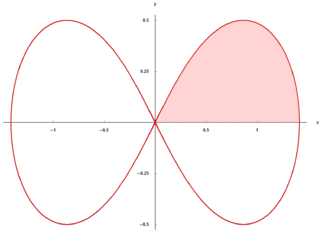
\includegraphics[width=0.8\textwidth]{img/Lemniscata.png}  
		\caption{La curva Lemniscata} 
		\label{figLemniscata}
	\end{center}  
\end{figure}


Estudiamos el área de uno de los cuadrantes al que llamamos $D$, el sombreado en la figura \ref{figLemniscata}, en el que la ecuación es $r = \sqrt{2} a \sqrt{\cos 2\theta}$. Su área sería

\[ 4\int\int_D dx\,dy = 4\int_0^{\frac{\pi}{4}} \int_0^{a\sqrt{2\cos 2\theta}} r \,dr\,d\theta = 4\int_0^{\frac{\pi}{4}} \frac{2a^2\cos 2\theta}{2} = 2a^2 \]

\subsection{Integración en $\real^3$}

La motivación para las integrales triples es el cálculo de la "masa" de región $\Omega$ con una densidad variable $f(x,y,z)$. La idea y la teoría es la misma que en dimensión dos, que nos acabará llevando a un teorema de Fubini (ver página \pageref{lblFubini}) y a un teorema de cambio de variable.

El primer problema que se plantea es cómo colocar los límites de integración. Tomaremos la función $f(x,y,z) = x^2\cos x$ y la región $T$ limitada (acotada) por los planos $z=0$, $z=\pi$, $x=0$, $y=0$ y $x+y = 1$, es decir, un prisma triangular (un prisma cuadrangular dividido por su diagonal).

La proyección de $T$ en el plano $XY$ es un triángulo, por lo que tomamos los límites en $x$ y en $y$ que nos dan esta región. Tendríamos entonces la siguiente integral:

\[ \int_0^1\int_0^{1-x} \int f\,dz\,dy\,dx \]

Observamos ahora el comportamiento de la variable $z$, que siempre valdrá $\pi$ independientemente de $x$ e $y$. La integral nos quedaría entonces de la siguiente forma:

\[ \int_0^1\int_0^{1-x} \int_0^{\pi} f\,dz\,dy\,dx \]

Vamos ahora a buscar los límites para una región más compleja, un paraboloide $z=x^2+y^2$ tapado por arriba por la esfera de radio 1 $x^2+y^2+z^2=1$. Primero hallamos la intersección entre ambas para encontrar la proyección en el plano $XY$. Sustituyendo, tenemos que $z+z^2 = 1$, por lo tanto y como $z>0$, tenemos que $z = \frac{\sqrt{5} -1}{2}$, de tal forma que la proyección sobre el plano $XY$ es la circunferencia de radio $R = \frac{\sqrt{5} -1}{2}$ centrada en el origen. De esta forma, la integral sería

\[ \int_{-R}^R \int_{-\sqrt{R^2-x^2}}^{\sqrt{R^2-x^2}}\int_{x^2+y^2}^{\sqrt{1-x^2-y^2}} f \, dz\,dy\,dx \]

\begin{theorem}[Cambio de variables en $\real^3$]
Dado un cambio de variables $\Phi(u,v,w) = (x(u,v,w), y(u,v,w), z(u,v,w)$, se transforma la integral

\[ \int\int\int_\Omega f(x,y,z)\,dx\,dy\,dz \]

en 

\[ \int\int\int_{\Omega*} f(\Phi(u,v,w)) \abs{\text{det}\left(\frac{∂(x,y,z)}{∂(u,v,w)}\right)}\,du\,dv\,dw \]

donde \[ \frac{∂(x,y,z)}{∂(u,v,w)} = \left(\begin{matrix}
\frac{∂x}{∂u} & \frac{∂x}{∂v} & \frac{∂x}{∂w} \\
\frac{∂y}{∂u} & \frac{∂y}{∂v} & \frac{∂y}{∂w} \\
\frac{∂z}{∂u} & \frac{∂z}{∂v} & \frac{∂z}{∂w} 
\end{matrix}\right) \]

\end{theorem}

\paragraph{Cambio a coordenadas cilíndricas}

Hacemos el cambio de variable a coordenadas cilíndricas, calculando el determinante

\[ \frac{∂(x,y,z)}{∂(u,v,w)} = \left|\begin{matrix}
\cos\theta & -r\sin\theta & 0\\
\sin\theta & r\cos\theta & 0 \\
0& 0 & 1
\end{matrix}\right| = r \]

\paragraph{Cambio a coordenadas esféricas}

Si calculamos el determinante, observamos cómo el cambio en la medida queda como $\rho^2\sin\varphi$.

\subsection{Integral\IS sobre curvas}
Imaginemos una curva $\Gamma \equiv \{ \sigma(t) = (x(t), y(t), z(t)),\, t\in [a,b]\}$. Sobre esta curva podemos hacer integrales de funciones escalares y de campos vectoriales.

\subsubsection{Integral de función escalar sobre una curva}

En este caso, nuestra curva $\Gamma$ es un alambre de densidad variable $f(x,y,z)$. Entonces, la integral sería la masa de ese alambre. No sabemos cómo hacer esta cuenta en el espacio, pero en el intervalo $[a,b]$ sí sabemos. Es decir, el problema es buscar una integral

\[ \int_a^b f(x(t), y(t), z(t))\,\ast\,dt \]

donde $\ast$ es el cambio en la medida. Para buscarlo, miramos qué ocurre cuando $f$ es constante y vale 1: la integral es la longitud de esa curva. Pero la longitud ya la hemos obtenido (ver \ref{refLong}), y sólo teníamos que integrar $\md{\sigma'(t)}$. De esta forma, nos quedaría que el cambio en la medida es $\md{\sigma'(t)}$ y la integral es 

\[ \int_a^b f(x(t), y(t), z(t))\,\md{\sigma'(t)}\,dt \]

\begin{theorem}
En el caso escalar, el resultado no depende de la parametrización.
\end{theorem}

\begin{proof}
Tenemos una curva $\Gamma$ con dos parametrizaciones: $\sigma_1(t)$, que transforma el intervalo $[a,b]$; y $\sigma_2(s)$ que lo hace con el $[c,d]$. Entonces, hay una biyección $h(t) = s$ que transforma el intervalo $[a,b]$ en $[c,d]$ y que es derivable $h$ y su inversa. Dada una función $f$, tendremos entonces que

\[ I = \int_\gamma f(x,y,z)\,d\sigma_2 = \int_c^df(\sigma_2(s))\md{\sigma_2'(s)}\,ds = \int_{h^{-1}(c)}^{h^{-1}(d)}f(\sigma_2(h(t)))\md{\sigma_2'(h(t))}h'(t)\,dt\]

Hay dos posibilidades sobre $h$: que sea decreciente o creciente. Si es creciente, transforma $[c,d]$ en $[a,b]$. Si es decreciente, tenemos que transforma $[c,d]$ en $[b,a]$.

Si $h$ es creciente, $h' ≥ 0$ por lo que $h = \abs{h}$. Entonces, nos queda que 

\[ I = \int_a^bf(\sigma_2(h(t)))\md{\sigma_2'(h(t))h'(t)}\,dt = \int_a^bf(\sigma_1(t))\md{\sigma_1'(t)}\,dt\].

Si $h$ es decreciente, $h' ≤ 0$ por lo que $-h = \abs{h}$. De esta forma, nos quedaría que

\[ I = \int_b^af(\sigma_2(h(t)))\md{\sigma_2'(h(t))}h'(t)\,dt = -\int_a^bf(\sigma_2(h(t)))\md{\sigma_2'(h(t))} h'(t)\,dt =\]\[= \int_a^bf(\sigma_2(h(t)))\md{\sigma_2'(h(t))h'(t)}\,dt \]
\end{proof}

\subsubsection{Integral de campo vectorial sobre una curva}

Aquí, la integral representa el trabajo realizado por el campo vectorial $\vec{F}$ alrededor de la curva $\Gamma$, más específicamente sobre la componente del vector tangencial a la curva en cada punto. A esta componente la llamaremos la componente efectiva. Una vez que calculamos esta componente, sólo tenemos números de forma que pasamos a una integral de función escalar.

Llamamos $\vec{v_t}$ al vector unitario tangente a la curva en un punto. Entonces, la componente efectiva $F_t = \md{\vec{F}} \cos \alpha$. Dado que $\vec{v_t}$ es de módulo uno, nos queda que $F_t = \pesc{\vec{F}, \vec{v_t}}$. De esta forma, concluimos que 

\[ \int_\Gamma \vec{F} \,d\sigma = \int_a^b \pesc{\vec{F}(\sigma(t)), \vec{v_t}} \md{\sigma'(t)}\,dt = \int_a^b \pesc{\vec{F}(\sigma(t)), \sigma'(t)} \,dt \]

\paragraph{Reparametrización}

Tenemos una curva $\Gamma$ con dos parametrizaciones: $\sigma_1(t)$, que transforma el intervalo $[a,b]$; y $\sigma_2(s)$ que lo hace con el $[c,d]$. Entonces, hay una biyección $h(t) = s$ que transforma el intervalo $[a,b]$ en $[c,d]$ y que es derivable $h$ y su inversa. De esta forma, $sigma_2(s) = \sigma_2(h(t)) = \sigma_1(t)$.

Hay dos posibilidades sobre $h$: que sea decreciente o creciente. Si es creciente, transforma $[c,d]$ en $[a,b]$. Si es decreciente, tenemos que transforma $[c,d]$ en $[b,a]$. En el primer caso, $h$ conserva la orientación y $\sigma_1$ y $\sigma_2$ tienen la misma orientación. En el caso decreciente, las parametrizaciones tienen distinta orientación.

\begin{theorem}
Si las dos parametrizaciones conservan la orientación sobre $\Gamma$, que es una curva simple o cerrada simple, entonces la integral mantiene el mismo valor. Si la orientación es distinta, las integrales son iguales con distinto signo.
\end{theorem}

\begin{defn}[Curva simple]\index{Curva!simple}
$\Gamma$ es una curva simple si la aplicación que la recorre es inyectiva.
\end{defn}

\begin{defn}[Curva cerrada simple]\index{Curva!cerrada simple}
$\Gamma$ es una curva cerrada simple si dada la aplicación $\appl{\sigma}{[a,b]}{\real^N}$ que la recorre, $\sigma$ es inyectiva en $[a,b)$ y $\sigma(a) = \sigma(b)$.
\end{defn}

\begin{proof}
Dada una función $F$, tendremos entonces que

\[ I = \int_\gamma F(x,y,z)\,d\sigma_2 = \int_c^d \pesc{F(\sigma_2(s)), \sigma_2'(s)}\, ds = \int_{\inv{h}(c)}^{\inv{h}(d)} \pesc{F(\sigma_2(h(t)), \sigma_2'(h(t))} h'(t) \,dt \]

Hay dos posibilidades sobre $h$: que sea decreciente o creciente. Si es creciente, transforma $[c,d]$ en $[a,b]$. Si es decreciente, tenemos que transforma $[c,d]$ en $[b,a]$.

Si $h$ es creciente, $h' ≥ 0$ por lo que $h = \abs{h}$. Entonces, nos queda que 

\[ I = \int_a^bf(\sigma_2(h(t)))\md{\sigma_2'(h(t))h'(t)}\,dt = \int_a^bf(\sigma_1(t))\md{\sigma_1'(t)}\,dt\].

Si $h$ es decreciente, $h' ≤ 0$ por lo que $-h = \abs{h}$. De esta forma, nos quedaría que

\[ I = \int_b^af(\sigma_2(h(t)))\md{\sigma_2'(h(t))}h'(t)\,dt = -\int_a^bf(\sigma_2(h(t)))\md{\sigma_2'(h(t))} h'(t)\,dt =\]\[ = \int_a^bf(\sigma_2(h(t)))\md{\sigma_2'(h(t))h'(t)}\,dt \]
\end{proof}

\subsubsection{Integrales en campos conservativos}

Si tenemos una curva $\Gamma \equiv \{\sigma(t) \tq t \in [a,b]\}$, la integral sobre el campo $F = \nabla U$ sería

\[ \int_\Gamma F = \int_a^b \pesc{F(\sigma(t)),\sigma'(t)}\,dt = \int_a^b \pesc{\nabla U (\sigma(t)),\sigma'(t)}\,dt = \]
\[ = \int_a^bDU(\sigma(t))D\sigma(t)\,dt = \int_a^b (U\circ\sigma)(t)dt = \left.(U\circ\sigma)(t)\right|_{t=a}^b \]

Es decir, en un campo conservativo la integral no depende del camino seguido, sólo de los puntos inicial y final:

\[ \int_\Gamma F = U(\sigma(b)) - U(\sigma(a)) \]

\subsection{Integrales sobre superficies}\index{Integral!sobre superficies}

\subsubsection{Integral de campo escalar sobre una superficie}

La motivación de la integral sobre una superficie es hallar la masa de una lámina con la forma $S$ y densidad superficial variable $f(x,y,z)$. La superficie $S$ se puede parametrizar a través de una aplicación $\Phi(u,v) = (x(u,v), y(u,v), z(u,v))$, donde $(u,v) \in D$. La integral se transforma entonces en

\[ \int\int_Sf(x,y,z) = \int\int_D f(\Phi(u,v))\ast \,du\,dv \]

donde, igual que antes, $\ast$ es el cambio en la medida. Para hallarlo, observamos qué ocurre cuando la densidad es constante y vale 1: deberíamos obtener el área de la superficie. Este área es la suma de todas las pequeñas áreas de $S$ que llamamos $S_{ij}$ y que obtenemos a partir de un rectángulo en la región $D$ que llamamos $R_{ij}$, de ancho $k$ y largo $n$.

El área de $S_{ij}$ es aproximadamente $\md{hT_u\x k T_v} = hk\md{T_u\x T_v}$, donde $T_u$ y $T_v$ son los vectores tangentes a la superficie $S_{ij}$ en el punto $(x(u_i, v_j), y(u_i, v_j), z(u_i, v_j)$. De esta forma, el área nos quedaría como

\[ \sum_{i,j}\md{T_u\x T_v} \text{Area}(R_{ij}) \]

que es una suma de Riemann para la función $\md{T_u\x T_v}$ en el plano $(u,v)$. De esta forma, la integral nos quedaría como 

\[ \int\int_D \md{T_u\x T_v}\,du\,dv \]

Por lo tanto

\[ \int\int_Sf(x,y,z) = \int\int_D f(\Phi(u,v))\md{T_u\x T_v} \,du\,dv \]

\paragraph{Ejemplos}

Probamos a obtener el área lateral de un \textbf{cilindro}, que debería ser $2\pi Rh$. En coordenadas cilíndricas, la parametrización sería \[\Phi(\theta, z) =(R\cos\theta, R\sin\theta, z)\;\theta\in [0,2\pi],\,z\in [0, h]\]

Hallamos los vectores $T_\theta =(-R\sin\theta, R\cos\theta, 0)$ y $T_z=(0,0,1)$. El producto vectorial valdría $(R\cos\theta, R\sin\theta,0)$ y su módulo vale $R$. La integral quedaría

\[ \int\int_S 1 = \int_0^h\int_0^{2\pi}R\,d\theta, dz = 2\pi Rh \]

Vamos ahora con la \textbf{esfera}, usando coordenadas esféricas. $T_\theta = (-R\sin\theta\sin\phi, R\cos\theta\sin\phi,0)$ y $T_\phi = ( R\cos\theta\cos\phi, R\sin\theta\cos\phi, -R\sin\phi)$. Entonces

\[ T_\theta\x T_\phi = -R^2\sin\phi(\cos\theta\sin\phi, \sin\theta\sin\phi,\cos\phi) \]

cuyo módulo vale $R^2\abs{\sin\phi}$. El área de la esfera sería entonces

\[ A = 8\int\int_S 1 = 8\int_0^{\pi /2}\int_0^{\pi /2} R^2\abs{\sin\phi}\,d\phi\,d\theta = 8R^2\int_0^{\pi/2}\left(-\cos\phi\right|_{\phi = 0}^{\pi /2} \,d\theta = \]
\[ = 8R^2\int_0^{\pi /2} 1\,d\theta = 8 R^2\frac{\pi}{2	} = 4\pi R^2\]

Probemos ahora con el \textbf{helicoide} (ver página \pageref{Helicoide}) de radio $R$, cuya parametrización es $\Phi(r,t) = (r\cos t, r\sin t, t)$. Hallamos los vectores tangentes $T_r = (\cos t, \sin t, 0)$ y $T_t=(-r\sin t, r\cos t, 1)$. El producto vectorial es $T_r\x T_t = (\sin t, -\cos t, r)$ y su módulo vale $\sqrt{1+r^2}$. El área sería entonces

\[ \int_0^R\int_0^2\pi = 2\pi\int_0^R\sqrt{1+r^2}\,dr \]

Para hallar la integral hacemos el cambio de variable $r = \sinh s$, de tal forma que $dr = \cosh s$. Quedaría entonces

\[ 2\pi \int_{\mathrm{arcsinh}(R)} \cosh^2 s \,ds  =  \frac{1}{2} (R \sqrt{1 + R^2}+ \textrm{arcsinh} (R)\]

\subsubsection{Integral de campo vectorial sobre una superficie}

Supongamos que $F$ es el campo de velocidades de un fluido que arrastra objetos. Ahora pensamos qué ocurre si colocamos una \textit{red}, que es una superficie $S$. La integral representa cuantos objetos \textit{capturamos} en la red por unidad del tiempo. Sin embargo, la parte efectiva del campo sólo es la componente normal del campo a la que llamamos $F_N$. De esta forma nos quedaría que

\[ \int\int_S\vec{F} = \int\int_D F_N \md{T_u\x T_v}\,du\,dv \]

Al igual que cuando hicimos para curvas, hallamos el vector normal como 

\[ F_N = \pesc{\vec{F}, \frac{T_u\x T_v}{\md{T_u\x T_v}} }\]

\subsection{Teoremas del análisis vectorial}

\begin{defn}[Orientación\IS positiva]
Dada una curva $\Gamma$, definimos su orientación positiva $\Gamma^+$. La obtenemos según la regla de la mano izquierda: nos colocamos de pie sobre la curva con la mano izquierda hacia el interior del dominio, de forma que nuestra nariz apunta a la orientación positiva de la curva.
\end{defn}

\begin{defn}[Orientaciones\IS compatibles]
Dada una curva $\Gamma$ y una superficie $S$, la orientación compatible $\Gamma^+$, $S^+$ es aquella en la que si nos colocamos de pie sobre la superficie en su vector normal, nos movemos hacia el borde de tal forma que la mano izquierda queda hacia dentro y la nariz apunta a la orientación compatible de la curva.\end{defn}


\begin{theorem}[Teorema\IS de Green]
Sea $\Gamma$ una curva simple en $\real^2$. Llamamos $D$ al interior de $\Gamma$. Sea $(P,Q)$ el campo con $P,Q\in C^1(D)$. Entonces

\[ \int_{\Gamma^+} (P,Q)\,d\sigma = \int\int_D \frac{\partial Q}{\partial x}-\frac{\partial P}{\partial y}\,dx\,dy\]
\end{theorem}

\begin{theorem}[Teorema de Stokes]\index{Teorema!de Stokes}
Dada $\Gamma$ una curva cerrada simple en $\real^3$ que es el borde de una superficie $S$, tenemos que 

\[ \int_{\Gamma^+}\vec{F}d\sigma =\int\int_{S^+}\rot \vec{F}dS \]

Esto indica que el flujo por una superficie depende sólo de la forma de su boca.
\end{theorem}

\begin{theorem}[Teorema\IS de Gauss]
Sea $S$ una superficie cerrada que encierra una región $\Omega$, y $\vec{F}\in C^1(\Omega)$.

\[ \int\int_{S^+} = \int\int\int_\Omega \dv \vec{F}\, dx\, dy\, dz \]
\end{theorem}

\printindex
\end{document}
